\documentclass{beamer}
\usetheme{Dresden}
%\usetheme{CambridgeUS}
\usepackage{helvet}
\usepackage{cite}
\usepackage{url}
\usepackage{amssymb, amsmath, graphicx, charter, latexsym}
\usepackage{subfigure}
\usepackage{enumerate}
\usepackage{ragged2e}
\usepackage{mathtools}
\usepackage{tabu}
\usepackage{epstopdf}
\usepackage{siunitx}
\renewcommand{\familydefault}{\sfdefault}
%\usepackage{times}
\setbeamertemplate{items}[circle]
\setbeamertemplate{navigation symbols}{}
\begin{document}
\title{Scheduling for Uplink Transmissions with Point Coordination Function}
\author{Dongni Han, Ping-Chun Hsieh, and Tao Zhao}
\date{April 28, 2016}
\newtheorem{thm}{Theorem}
\begin{frame}
\titlepage
\end{frame}


%\begin{frame}
%\frametitle{What to Discuss Today?}
%\tableofcontents[]
%\end{frame}

%\AtBeginSection[]
%{
	%\begin{frame}{Table of Contents}
	%\tableofcontents[currentsection]
	%\end{frame}
%}

\NewDocumentCommand{\varSI}{O{}}{\SI[detect-all=true,parse-numbers=false,#1]}

\section{Background}

\begin{frame}
\frametitle{System Model}
\begin{itemize}
  \item WiFi network
    \begin{itemize}
      \item One AP and $N$ clients
      % \varSI must be outside math env for it to have right font family.
      \item $\SI{1}{slot} = \SI{10}{ms}$; $\SI{1}{interval} =$ \varSI{T}{slots}
    \end{itemize}
  \item Uplink Transmissions
    \begin{itemize}
      \item Packets generated at each client $n$ in each interval $k$
      \item Number of packets $a_n(k)$ follows Unif$\{U_\text{min}, U_\text{max}\}$
      \item Real-time traffic
    \end{itemize}
  \item Point Coordination Function (PCF)
    \begin{itemize}
      \item AP polls (at most) one client per slot
      \item But AP needs to know $a_n(k)$ first!
    \end{itemize}
\end{itemize}
\end{frame}

\begin{frame}
\frametitle{Baseline Policy: Phase 1}
\begin{itemize}
\item AP polls $a_n(k)$ for all $n$ one by one
\end{itemize}
\begin{figure}
\centering
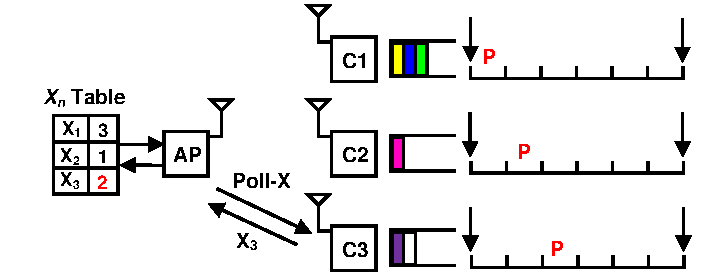
\includegraphics[scale=0.8]{animation_03.pdf}
\end{figure}
\end{frame}

\begin{frame}
\frametitle{Baseline Policy: Phase 2}
\begin{itemize}
\item AP uses Max-Weight scheduling for data transmissions
\end{itemize}
\begin{figure}
\centering
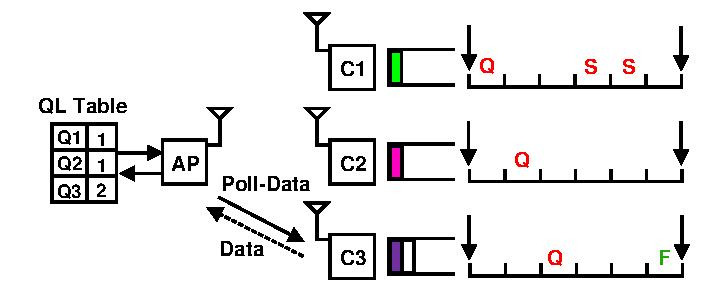
\includegraphics[scale=0.8]{animation_06.pdf}
\end{figure}
\end{frame}

\begin{frame}{Baseline Policy: Issues}
  \begin{itemize}
    \item No data transmissions in Phase 1
    \item Huge overhead especially with large $N$ and bad channels
    \item We need a smarter policy!
  \end{itemize}
\end{frame}
\section{Smart Policy}

\begin{frame}
\frametitle{Idea 1: Selective Scheduling}
\begin{itemize}
\item Only schedule $n \le N$ clients per interval
\item Random permutation for fairness and stability
\item Schedule remaining clients only after all selected are scheduled
\end{itemize}
\end{frame}


\begin{frame}
\frametitle{Feature 001: Selective Scheduling}
\begin{itemize}
\item How to determine the optimal $n$?
  \begin{itemize}
    \item Sort clients by channel reliabilities $p_1 > p_2 > \dots > p_N$
    \item Estimated throughput: $\hat{R}_n = \min\{n, (T-\sum_{i=1}^{n}\frac{1}{p_i})\frac{\sum_{i=1}^{n}p_i}{n} \}$
      %fixme
    %\item Find the optimizer $n = \argmax \hat{R}_n$
  \end{itemize}
\item Random permutation?
  \begin{itemize}
    \item Classic problem: random poker shuffling (Knuth)
  \end{itemize}
\item How to schedule remaining clients?
  \begin{itemize}
    \item Greedy: poll $a_n(k)$ and data one by one
  \end{itemize}
\end{itemize}
\end{frame}

\begin{frame}
\frametitle{Discussion 3}
\begin{itemize}
\item For non-real-time traffic, what does "$X_n$" mean? 
\item There is no application-layer ACK from AP
\end{itemize}
\begin{figure}
\centering
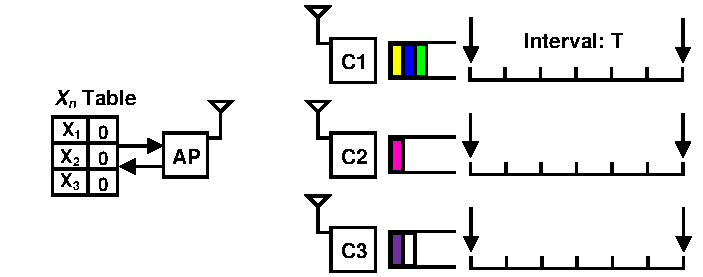
\includegraphics[scale=0.65]{discussion_3.pdf}
\end{figure}
\pause
\begin{itemize}
\item $X_n:=$ total number of packets generated by client $n$
\item $Y_n:=$ total delivery of data packets from client $n$ (maintained by AP)
\item Max-Weight: choose $n$ that maximizes $p_n(X_n-Y_n)$
\end{itemize}
\end{frame}

\begin{frame}
\frametitle{NS-2 Implementation: Packet Types}
\begin{itemize}
\item AP: {\color{red}{Poll-X}} and {\color{red}{Poll-DATA}}
\item Client: {\color{red}{X-Uplink}} and {\color{red}{DATA-Uplink}}
\end{itemize}
\begin{figure}
\centering
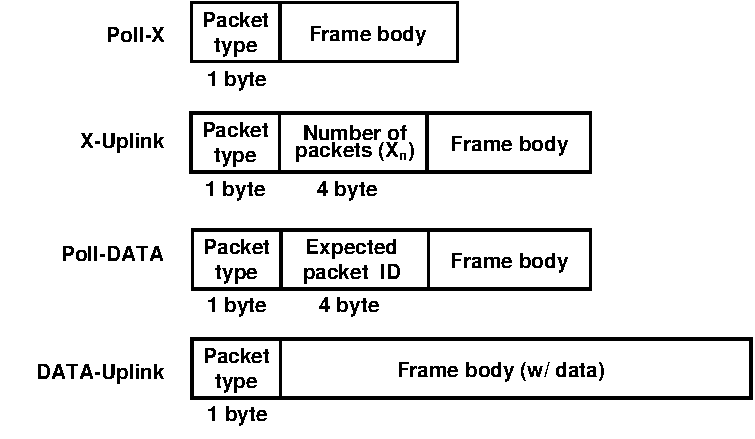
\includegraphics[scale=0.7]{header.pdf}
\end{figure}
\end{frame}

\begin{frame}
\frametitle{NS-2 Implementation: State Machine}
\begin{itemize}
\item AP is controlled by the state machine as follows.
\end{itemize}
\begin{figure}
\centering
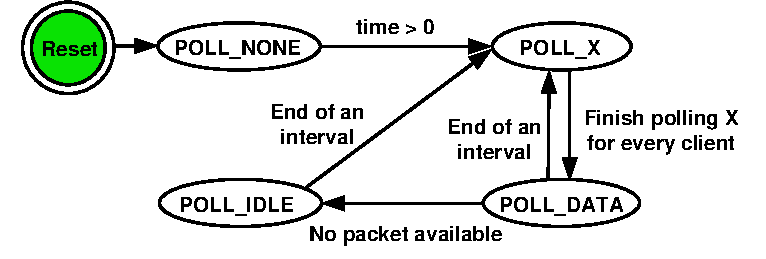
\includegraphics[scale=0.8]{state_machine.pdf}
\end{figure}
\end{frame}


\begin{frame}
\frametitle{Pros and Cons}
\color{blue}{Pros:}
\begin{itemize}
\item Simple polling scheme
\item AP is work-conserving in phase 2 
\end{itemize}
\color{blue}{Cons:}
\begin{itemize}
\item Overhead due to polling
\item Channel utilization for data packets is low
\item Not practical when $N$ is large
\end{itemize}
\end{frame}


\section{Simulation}

\begin{frame}
\frametitle{Simulation Results: Network Capacity}
\begin{itemize}
\item $N=2$ and $T=10$
\item Reliable channel: $p_1 = p_2 = 1$ (symmetric)
\item $N_\text{max}$ ranges from $1$ to $12$
\item Non-real-time traffic
\end{itemize}
\begin{figure}
\centering
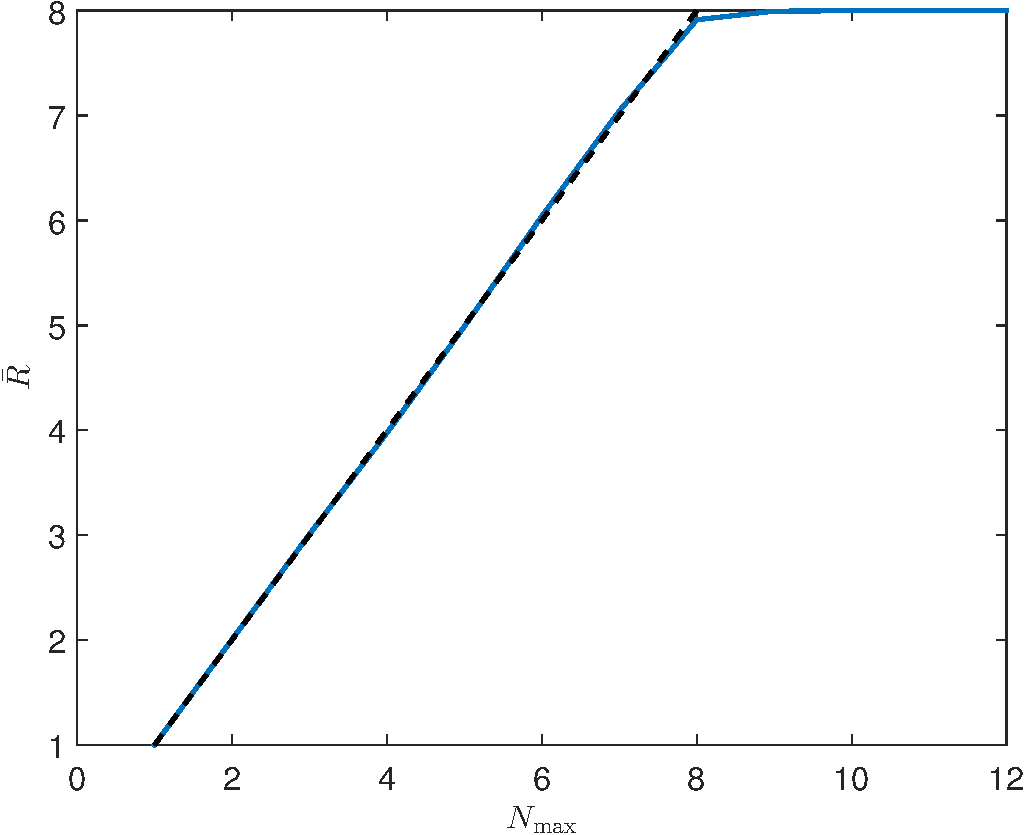
\includegraphics[height=.5\textheight]{nonrealtime_throughput_randmax.pdf}
\caption{Phase 1 polling reduces the capacity.}
\end{figure}
\end{frame}

\begin{frame}
\frametitle{Simulation Results: Network Capacity}
\begin{itemize}
\item $N=2$ and $T=10$
\item Reliable channel: $p_1 = p_2 = 1$ (symmetric)
\item $N_\text{max}$ ranges from $1$ to $20$
\item Real-time traffic
\end{itemize}
\begin{figure}
\centering
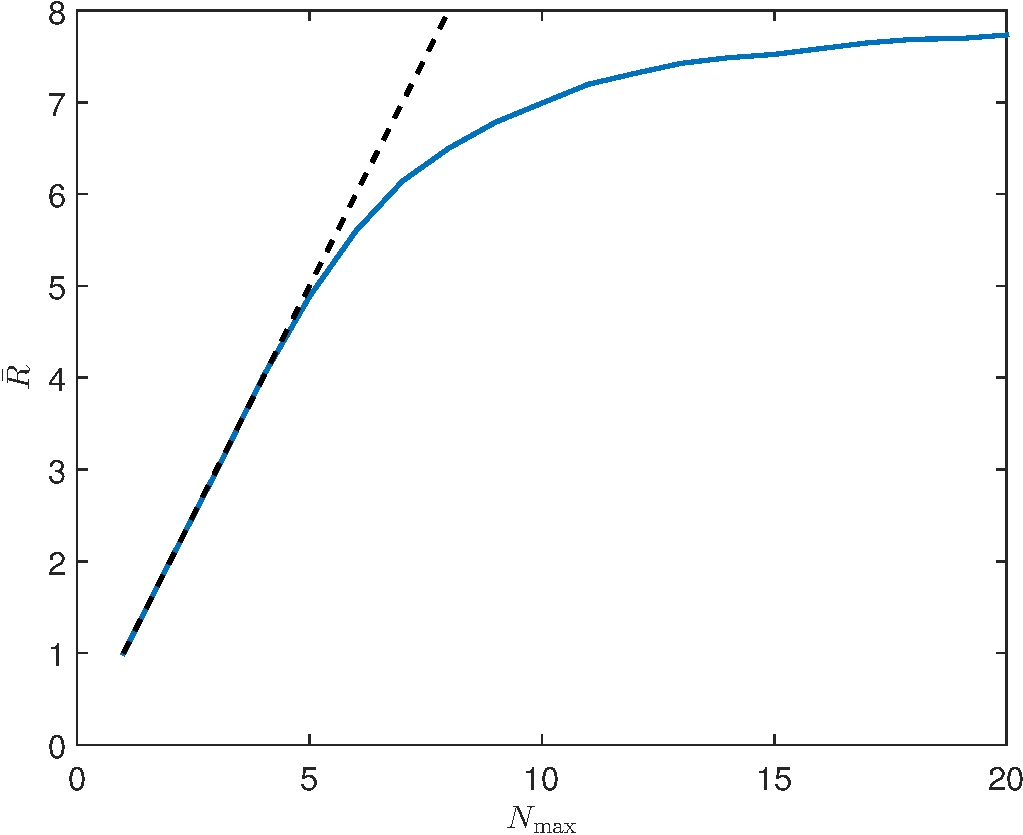
\includegraphics[height=.5\textheight]{realtime_throughput_randmax.pdf}
\caption{Packet deadline reduces the capacity further.}
\end{figure}
\end{frame}

\begin{frame}
\frametitle{Simulation Results: Interval Length}
\begin{itemize}
\item $N=2$
\item Unreliable channel: $p_1 = p_2 \approx 0.57$ (distance \SI{1000}{m})
\item $T$ ranges from $4$ to $16$
\item Non-real-time traffic
\end{itemize}
\begin{figure}[htbp]
  \centering
  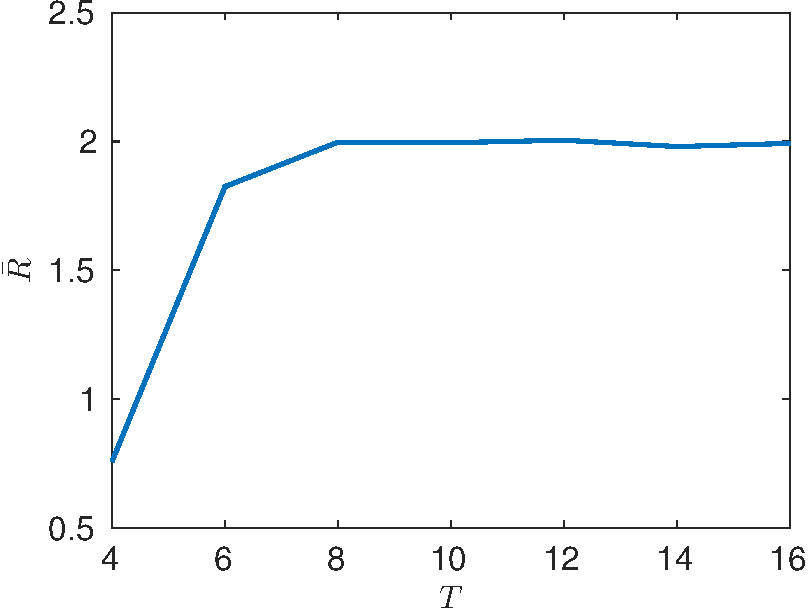
\includegraphics[height=.5\textheight]{nonrealtime_throughput_T.pdf}
  \caption{Interval should be long enough to guarantee deliveries.}
\end{figure}
\end{frame}

\begin{frame}
\frametitle{Simulation Results: Interval Length}
\begin{itemize}
\item $N=2$
\item Unreliable channel: $p_1 = p_2 \approx 0.57$ (distance \SI{1000}{m})
\item $T$ ranges from $4$ to $16$
\item Real-time traffic
\end{itemize}
\begin{figure}[htbp]
  \centering
  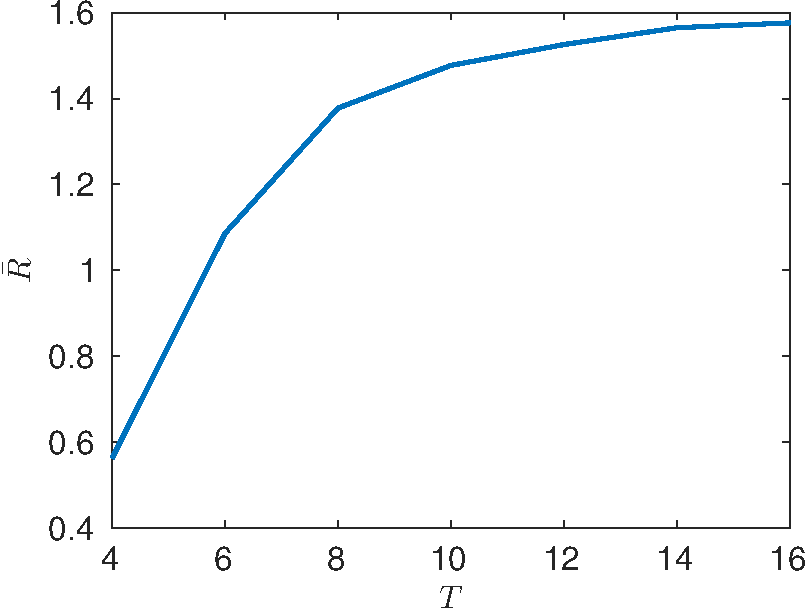
\includegraphics[height=.5\textheight]{realtime_throughput_T.pdf}
  \caption{Interval should be longer when packet can expire.}
\end{figure}
\end{frame}

\begin{frame}
\frametitle{Simulation Results}
\begin{itemize}
  \item Fix $T=10$
\item Unreliable channel: $p_1 = p_2 \approx 0.57$ (distance \SI{1000}{m})
\item $N$ ranges from $1$ to $5$
\item Non-real-time traffic
\end{itemize}
\begin{figure}[htbp]
  \centering
  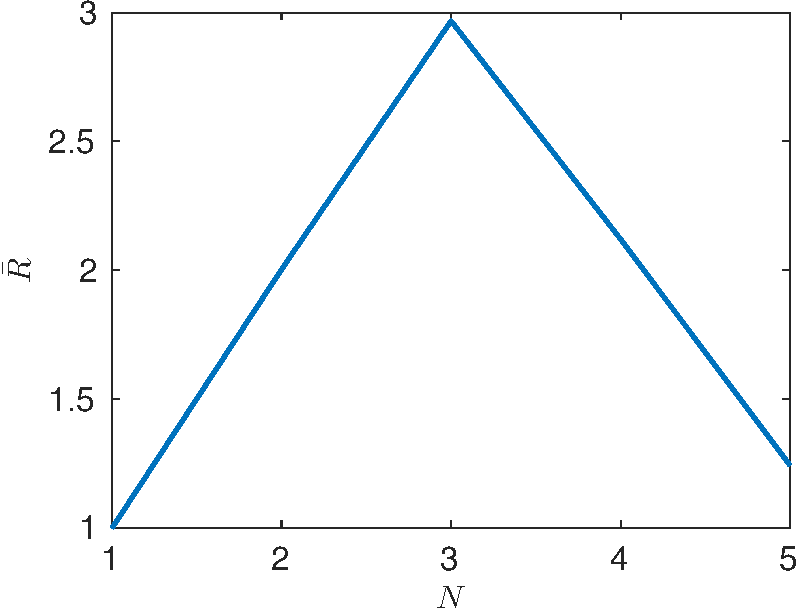
\includegraphics[height=.5\textheight]{nonrealtime_throughput_N.pdf}
  \caption{Performance degrades severely with more clients.}
\end{figure}
\end{frame}

\begin{frame}
\frametitle{Simulation Results}
\begin{itemize}
  \item Fix $T=10$
\item Unreliable channel: $p_1 = p_2 \approx 0.57$ (distance \SI{1000}{m})
\item $N$ ranges from $1$ to $5$
\item Real-time traffic
\end{itemize}
\begin{figure}[htbp]
  \centering
  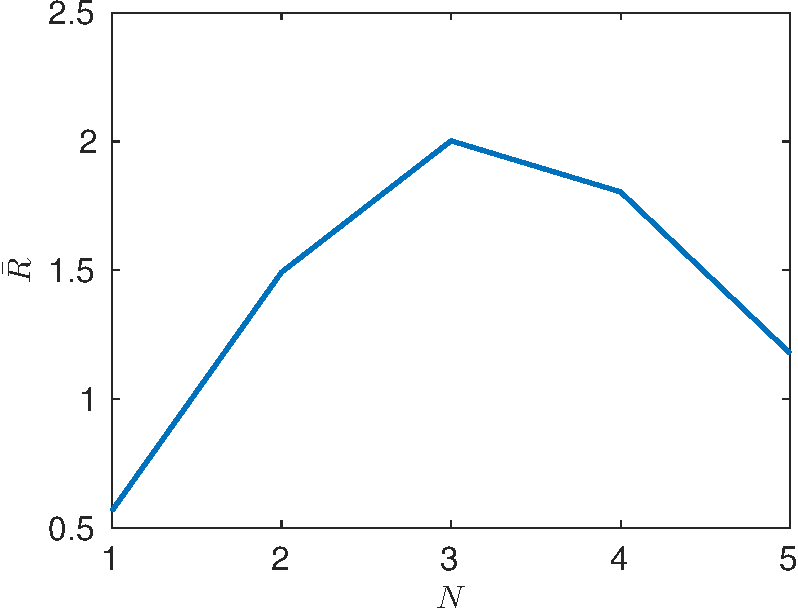
\includegraphics[height=.5\textheight]{realtime_throughput_N.pdf}
  \caption{Performance is worse and also degrades with more clients.}
\end{figure}
\end{frame}

\section*{Conclusion}
\begin{frame}{Conclusion}
  \begin{itemize}
    \item The baseline policy incurs huge overhead especially with large $N$ and small $T$
    \item We need a smarter policy!
  \end{itemize}
\end{frame}


\end{document}
